\subsection{Mechanistic Model and Experimental Data}
\subsubsection{Base Mechanistic Model and Calibration Dataset}
The mechanistic model used for EnKF implementation was adapted from the cell culture framework described by Kotidis \textit{et al.} (2019) \cite{Kotidis2019Model-basedCulture}, with model equations provided in Supplementary Information ~\ref{model}. This reduced model captures key extracellular dynamics, including cell growth and death, metabolism, and antibody synthesis, while excluding intracellular modules related to nucleotide sugar metabolism and glycosylation. The experimental data for this mechanistic model calibration were obtained from fed-batch cultures of an IgG-producing CHO-T127 cell line. The culture were maintained in CD CHO medium (Life Technologies, Paisley, UK) at 36.5°C with 5\% CO\textsubscript{2} and agitated at 150 rpm. Cells were passaged every 3-4 days, with 50 $\mu$M of methionine sulfoximine supplemented during the initial two passages after revival. Cultures were grown in 500 mL vented Erlenmeyer flasks (Corning, Amsterdam, The Netherlands) with a 100 mL working volume and an initial seeding density of 2 × 10\textsuperscript{5} cells mL\textsuperscript{-1}. 10\% (v/v) CD EfficientFeed C™ C AGT™ (Life Technologies, Paisley, UK) was added every alternate day starting from day 2 \cite{Kotidis2019Model-basedCulture}.

\begin{table}[ht]
    \centering
    \small % keep readable size
    \renewcommand{\arraystretch}{1.3} % was 2, slightly tighter
    \setlength{\tabcolsep}{5pt} % was 7pt, narrower columns
    \caption{Summary of experimental datasets. Only the feed concentration of nutrients considered in the model is reported. *Dataset~3 operates at 36.5\textdegree C before a downshift to 32\textdegree C on day~6.}
    \label{tab:datasets}
    \begin{tabular}{l l c c c c c c c l}
        \toprule
        \textbf{\#} & \textbf{\makecell{Cell\\Line}} & \multicolumn{3}{c}{\textbf{Bioreactor}} & \multicolumn{3}{c}{\textbf{Feed Concentration (mM)}} & \textbf{Ref} \\
        \cmidrule(lr){3-5} \cmidrule(lr){6-8}
         &  & \textbf{Type} & \textbf{Volume (mL)} & \textbf{Temp (°C)} & \textbf{Glc} & \textbf{Glu} & \textbf{Asn} & \\
        \midrule
        1 & A   & Shake flask  & 100 & 36.5 & 144.4 & 12.2 & 27.0 & \cite{Kotidis2019Model-basedCulture} \\
        2 & A   & Bioreactor   & 900 & 36.5 & 144.4 & 12.2 & 27.0 & \cite{Sou2015HowGlycosylation} \\
        3* & A  & Bioreactor   & 900 & 32   & 144.4 & 12.2 & 27.0 & \cite{Sou2015HowGlycosylation} \\
        4 & B   & Shake flask  & 50  & 36.5 & 144.4 & 12.2 & 27.0 & \cite{Kyriakopoulos2014ACulture} \\
        5 & B   & Shake flask  & 50  & 36.5 & 144.4 & 21.4 & 73.6 & \cite{Kyriakopoulos2014ACulture} \\
        6 & B   & Shake flask  & 50  & 36.5 & 202.2 & 29.9 & 103.1 & \cite{Kyriakopoulos2014ACulture} \\
        \bottomrule
    \end{tabular}
\end{table}

To investigate whether the EnKF can adapt a fixed mechanistic model beyond its original parametrisation, we applied the method to datasets from diverse bioprocess conditions. These included changes in bioreactor scale, temperature, host cell line, and feeding strategy, as summarised in Table~\ref{tab:datasets}. The structure of the model remained unchanged across all cases, with only model \rev{parameters} updated recursively during the culture.

\subsubsection{Same Cell Line: Scale and Temperature Variation}
The first three datasets correspond to the same CHO-T127 cell line (Cell Line A). Dataset 1 represents the original shake-flask culture used for model calibration, whereas Datasets 2 and 3 were conducted in 1.5 L stirred-tank bioreactors (DASGIP Technology, Jülich, Germany) to evaluate model transferability across scales and temperature conditions. Both bioreactor datasets were seeded at 8 × 10\textsuperscript{5} cells mL\textsuperscript{-1} with a working volume of 0.9 L and maintained at pH 6.9 $\pm$ 0.1, 5\% CO\textsubscript{2}, 150 rpm agitation, and active antifoam control. In Dataset 2, the culture temperature was held constant at 36.5 °C, while in Dataset 3, a temperature downshift from 36.5 °C to 32 °C was introduced on day 6. The bioreactor cultures followed the same feeding schedule as the shake-flask experiment, with 10\% (v/v) of Feed C added on even-numbered days starting on day 2, and were further supplemented with 10\% (v/v) of a proprietary nutrient Feed X (MedImmune, Cambridge, UK) \cite{Sou2015HowGlycosylation}.

\subsubsection{Different Cell Line: Feeding Strategy Variation}
To evaluate the capability of EnKF to support cross-cell line knowledge transfer, three additional datasets based on CHO-GS46 (Cell Line B) were tested, each employing a distinct feeding strategy. Cultures were incubated in 250 mL Erlenmeyer flasks (Corning, Amsterdam, The Netherlands) with a 50 mL working volume, incubated at 36.5°C, 140 rpm, and 8\% CO\textsubscript{2}. Feeding was performed every other day using a tenfold-concentrated nutrient supplement at 10\% (v/v). Dataset 4 employed the same commercial feed used in Cell Line A shake flask culture. Datasets 5 and 6 used in-house formulations Feed U and Feed U plus 40\%, developed from the batch culture nutrient consumption profiles of Cell Line B. Amino acid and glucose concentrations were scaled to sustain a threefold increase in integrated viable cell concentration, with the latter formulation containing 40\% higher nutrient levels except for tyrosine, which was limited by solubility. While the feeds contained a broader range of components, only the nutrients represented in the model are listed in Table~\ref{tab:datasets} \cite{Kyriakopoulos2014ACulture}.

\subsubsection{Analytical Methods}
Cell concentration and viability were measured either manually using a Neubauer haemocytometer with trypan blue exclusion for shake flask samples or with the automated ViCell® system (Beckman Coulter, CA) for bioreactor cultures. Antibody titre in shake flask samples was quantified using the BLItz® system with Dip and Read™ Protein A biosensors (Pall ForteBio, Portsmouth, UK), whereas in the bioreactor studies, secreted mAb concentration was determined by Protein A affinity chromatography. Extracellular glucose, glutamine, glutamate, lactate, and ammonia concentrations were measured using the BioProfile 400 analyser (NOVA Biomedical, MA) for shake flask experiments , while bioreactor samples were analysed using the YSI Bioprofiler 800 (NOVA Biomedical, MA). Extracellular amino acid concentrations, including asparagine, were quantified by high-performance or ultra-performance liquid chromatography (HPLC/UPLC, Waters, Hertfordshire, UK) using the AccQ-Tag™ kit according to the manufacturer’s protocol.

\subsection{EnKF Dual State and Parameter Estimation}
Figure~\ref{fig:enkf_schematic} illustrates the structure and information flow of the dual EnKF implementation. At each update step, ensembles of parameters and states, initially sampled from prior distributions, are propagated through the mechanistic model. As new measurements become available, the parameter and state ensembles are sequentially updated, reducing their spread and thereby the associated uncertainty. The narrowing of these distributions reflects convergence towards the true system dynamics, enabling continuous refinement of both parameters and states throughout the culture.


The ensemble is initialised at $t = 0$ with \rev{$N$} members, each obtained by independently sampling the state and parameter vectors from Gaussian distributions centred at their prior nominal values, thereby generating \rev{$N$} distinct realisations that collectively represent the prior uncertainty:
\setlength{\abovedisplayskip}{3pt}
\setlength{\belowdisplayskip}{3pt}
\begin{equation}
{\color{blue}x_{t=0}^i\sim \mathcal{N}(x_{t=0}, P_{t=0}^{xx}), \quad
\theta_{t=0}^i\sim \mathcal{N}(\theta_{t=0},P_{t=0}^{\theta\theta})}
\label{state_ensemble}
\end{equation}
where $x_t^i \in \mathbb{R}^{n_x}$ is the state vector and $\theta_t^i \in \mathbb{R}^{n_\theta}$ is the parameter vector for the $i$th ensemble member, and $i = 1,2,\dots,\rev{N}$. Superscripts $-$ and $+$ denote \rev{pre- and post-measurement update} estimates, respectively. \rev{$P_{t=0}^{xx} \in \mathbb{R}^{n_x \times n_x}$ and $P_{t=0}^{\theta\theta} \in \mathbb{R}^{n_\theta \times n_\theta}$ denote the initial state and parameter covariance matrices, respectively. The process noise covariance $Q \in \mathbb{R}^{n_x \times n_x}$ captures process uncertainties, while the measurement noise covariance $R \in \mathbb{R}^{n_x \times n_x}$ represents observation uncertainty. Here, all eight state variables are measured at each sampling time, so the observation operator is the identity ($H = I_{n_x}$) and $n_z = n_x$ throughout. }

\begin{figure}[H]
    \centering
    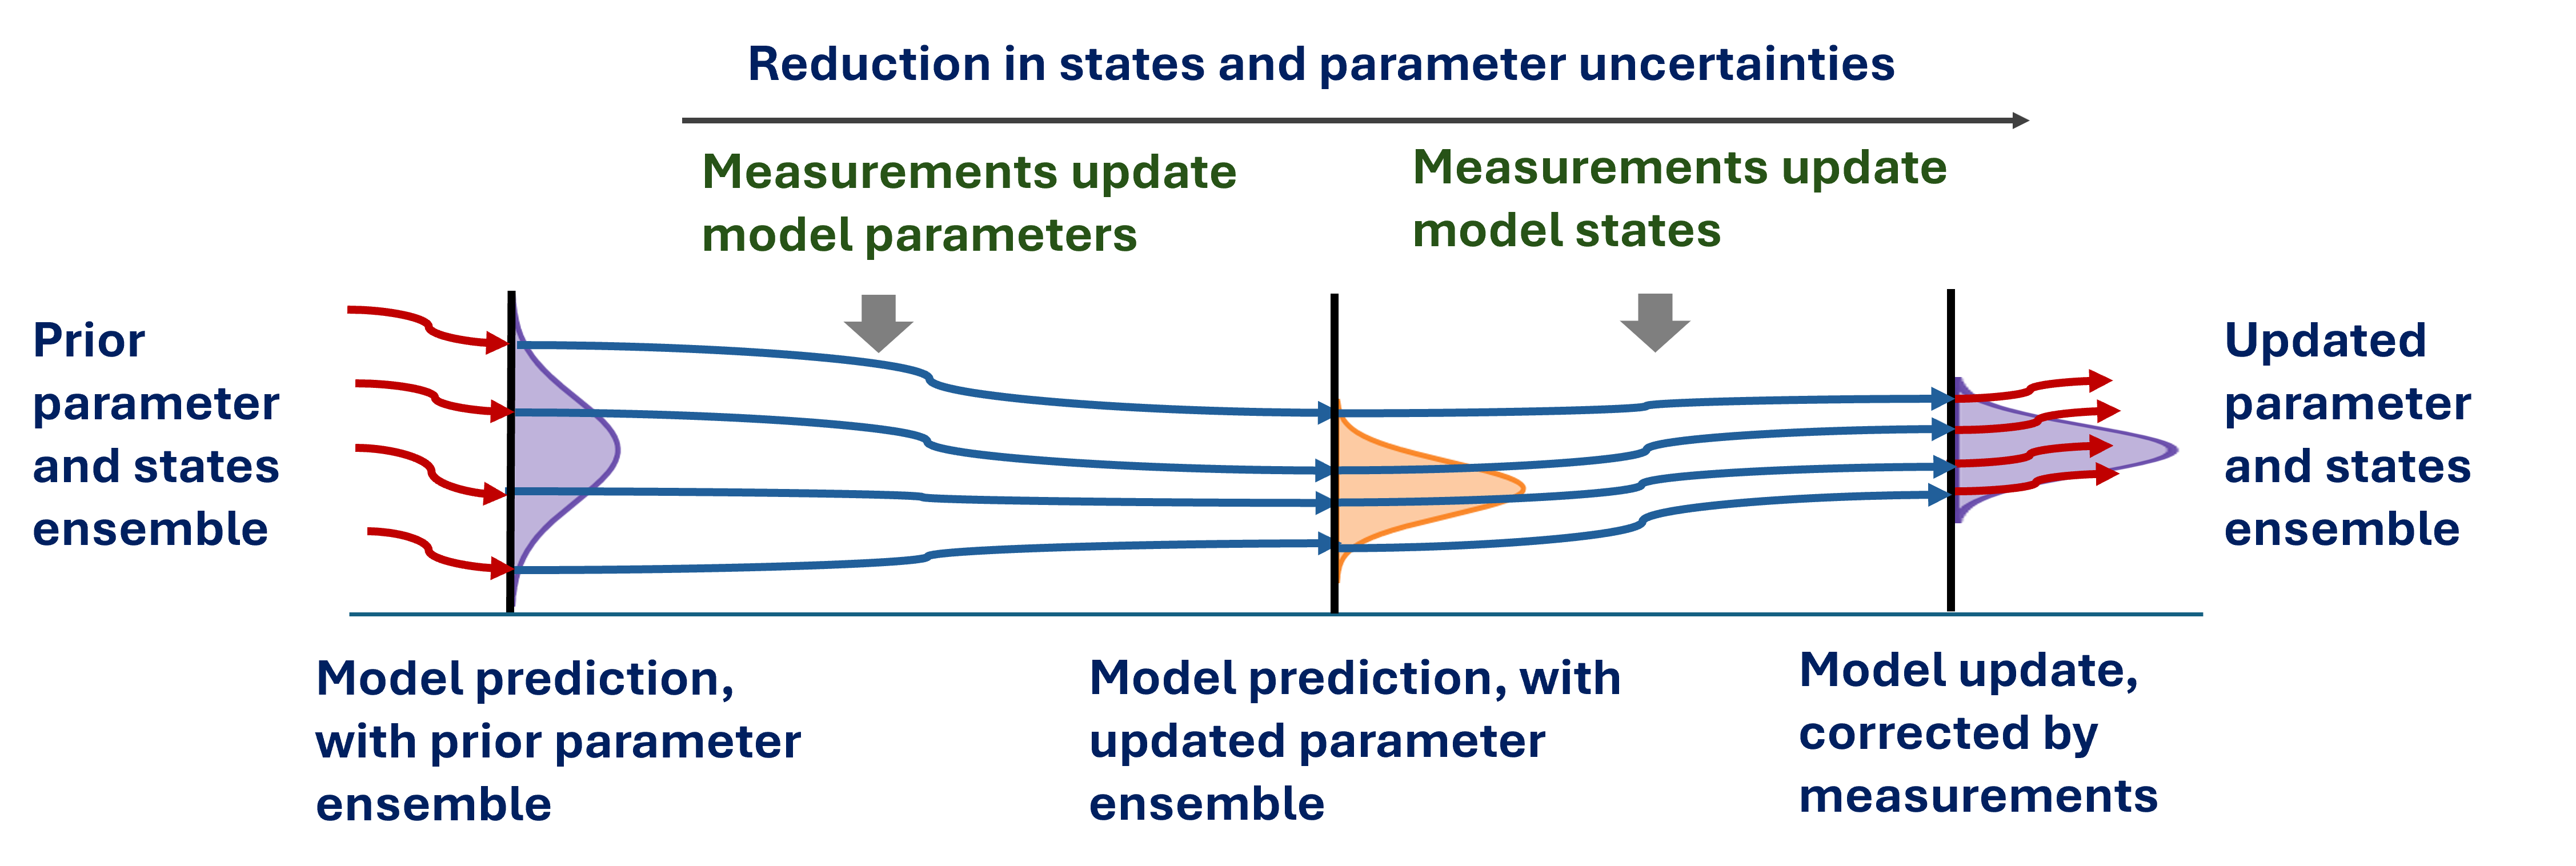
\includegraphics[width=0.95\textwidth]{Figs/enkf_schematic.png}
    \caption{\rev{Schematic of the dual EnKF framework for state and parameter estimation. Ensembles of model states and parameters, initialised from prior distributions, are propagated through the mechanistic model and sequentially updated upon arrival of new measurements, progressively reducing uncertainty and refining both state and parameter estimates throughout the culture.}}
    \label{fig:enkf_schematic}
    \end{figure} 
    


The mechanisticmodel used in this study is based on Kotidis \textit{et al.} (2019), with published parameter values used as the prior mean. For each dataset, the initial ensemble covariance reflects dataset-specific uncertainty in parameters and states. The ensemble of prior states evolves through the model using the prior parameter ensemble, with Gaussian-distributed process noise added to account for model uncertainty:
\begin{equation}
{\color{blue}x_{t+1}^{i-}=f\left(x_t^{i+},\theta_{t+1}^{i-}\right)+\varepsilon_t^i,\quad
\varepsilon_t^i\sim \mathcal{N}(0, Q)}
\label{prior_pred}
\end{equation}


The model is numerically integrated with a fine internal time step to capture system dynamics continuously, while measurement updates occur only when experimental data become available, typically once per day in fed-batch cultures. When off-line measurements are obtained, the reported experimental mean is used as the central value, and an observation ensemble is generated to reflect the associated measurement uncertainty \cite{Evensen2022DataProblem}:
\setlength{\abovedisplayskip}{3pt}
\setlength{\belowdisplayskip}{3pt}
\begin{equation}
{\color{blue}z_{t+1}^i \sim \mathcal{N}\bigl(z_{t+1}, R\bigr)}
\label{obs_rep}
\end{equation}
where $z_{t+1}^i$ denotes the $i$th perturbed measurement. The experimental error bar can be used as a practical reference for \rev{$R$}, accounting \rev{for} sampling and instrument uncertainty. \rev{A lower bound of zero is enforced on each perturbed observation to prevent non-physical negative concentrations.} The measurements are then used to correct the model parameter ensemble. The parameter update follows the standard Kalman correction: 
\begin{equation}
\theta_{t+1}^{i+}=\theta_{t+1}^{i-}+K_{t+1}^\theta\left(z_{t+1}^i-x_{t+1}^{i-}\right)
\label{para_update}
\end{equation}
The update is scaled by the parameter Kalman gain $K_{t+1}^\theta$, which determines how strongly each parameter is adjusted based on the current mismatch between model prediction and measurement.
\setlength{\abovedisplayskip}{3pt}
\setlength{\belowdisplayskip}{3pt}
\begin{equation}
{\color{blue}K_{t+1}^\theta = P_{t+1}^{\theta x}\bigl(P_{t+1}^{xx} + R\bigr)^{-1}}
\label{para_Kgain}
\end{equation}
\rev{where $P_{t+1}^{\theta x}$ is the cross-covariance between the parameter and predicted state ensembles, and $P_{t+1}^{xx}$ is the predicted state error covariance, both estimated as sample statistics from the ensemble:}
\begin{equation}
{\color{blue}P_{t+1}^{\theta x} = \frac{1}{N-1}\sum_{i=1}^{N}\bigl(\theta_{t+1}^{i-} - \bar{\theta}_{t+1}^{-}\bigr)\bigl(x_{t+1}^{i-} - \bar{x}_{t+1}^{-}\bigr)^{\!\top}\!, \quad
P_{t+1}^{xx} = \frac{1}{N-1}\sum_{i=1}^{N}\bigl(x_{t+1}^{i-} - \bar{x}_{t+1}^{-}\bigr)\bigl(x_{t+1}^{i-} - \bar{x}_{t+1}^{-}\bigr)^{\!\top}}
\label{eq:sample_cov}
\end{equation}
\rev{where $\bar{\theta}_{t+1}^{-}$ and $\bar{x}_{t+1}^{-}$ denote the ensemble means of the predicted parameters and states, respectively.} The updated parameter ensemble is then used to re-predict the states:
\begin{equation}
{\color{blue}x_{t+1}^{i-}=f\left(x_t^{i+},\theta_{t+1}^{i+}\right)+\varepsilon_t^i,\quad
\varepsilon_t^i\sim \mathcal{N}\left(0, Q\right)}
\label{posterior_pred}
\end{equation}
The predicted states are subsequently corrected using the \rev{state} Kalman gain $K_{t+1}^x$, which balances the confidence in the model prediction against the reliability of the experimental data.
\begin{equation}
x_{t+1}^{i+} = x_{t+1}^{i-} + K_{t+1}^x(z_{t+1}^i - x_{t+1}^{i-})
\label{state_update}
\end{equation}
\begin{equation}
{\color{blue}K_{t+1}^x = P_{t+1}^{xx} (P_{t+1}^{xx} + R)^{-1}}
\label{states_gain}
\end{equation}


In this work, a dual estimation structure was adopted instead of a fully joint formulation in which states and parameters are concatenated into a single augmented vector. In the state update, stochastic process noise is explicitly introduced at each propagation step to capture model uncertainty, effectively inflating the covariance matrix dynamically. For parameters, no artificial noise is injected, ensuring that changes in ensemble spread reflect genuine information gain from experimental data rather than covariance inflation. By maintaining separate ensembles, state propagation remains numerically stable while parameter evolution can retain a relatively large initial covariance to permit adaptive learning. If a large initial covariance were assigned to the augmented state-parameter vector, the resulting integration would become computationally unstable and inefficient due to the need for repeated numerical integration with overly dispersed trajectories. This separation therefore facilitates both stable computation and biologically interpretable parameter trajectories. \rev{The complete sequential update procedure is summarised in Figure~\ref{fig:enkf_workflow}.}

\begin{figure}[H]
    \begin{center}
    \begin{adjustbox}{max width=\textwidth, max height=0.85\textheight}
        \begingroup
        \setstretch{1.3}
        \begin{tikzpicture}[every node/.style={font=\scriptsize}, xscale=1.5]
        
          \def\nodespacing{.3cm}
          \def\decisionwidth{4cm}
          \def\decisionaspect{3}
          \def\processwidth{5.5cm}
          
          % Nodes
          \node (start) [startstop] {Initialize};

          \node (step2) [process, below=\nodespacing of start.south] 
          {Create state and parameter ensembles of size ${\color{blue}N}$ with their corresponding covariance:\\ $x_{t=0}^i,\, \theta_{t=0}^i\sim \mathcal{N}\!\left([x_{t=0},\, \theta_{t=0}]^T,\,\mathrm{diag}\!\left({\color{blue}P_{t=0}^{xx}},\, {\color{blue}P_{t=0}^{\theta\theta}}\right)\right),\quad i = 1,2, \dots,{\color{blue}N}$};

          \node (step3) [process, below=\nodespacing of step2.south] 
          {Model prediction of states with available mechanistic model: $x_{t+1}^{i-}=f\left(x_t^{i+},\theta_{t+1}^{i-}\right)+\varepsilon_t^i,\ \ \ \ \varepsilon_t^i\sim \mathcal{N}(0,{\color{blue}Q})$};

          \newdimen\ysouththree
          \newdimen\xeastthree
          \newdimen\ycenterthree
          \newdimen\heightthree
          \pgfextracty{\ysouththree}{\pgfpointanchor{step3}{south}}
          \pgfextractx{\xeastthree}{\pgfpointanchor{step3}{east}}
          \pgfextracty{\ycenterthree}{\pgfpointanchor{step3}{center}}
          \pgfextracty{\heightthree}{\pgfpointdiff{\pgfpointanchor{step3}{north}}{\pgfpointanchor{step3}{south}}}

          \node (step31) [decision, minimum width=\decisionwidth, aspect=\decisionaspect, below=\nodespacing of step3.west, xshift=\decisionwidth/2, yshift=\heightthree/2] 
          {Measurement available?};

          \newdimen\xnorththreeone
          \newdimen\ynorththreeone
          \newdimen\ysouththreeone
          \newdimen\heightthreeone
          \newdimen\ycenterthreeone
          \pgfextractx{\xnorththreeone}{\pgfpointanchor{step31}{north}}
          \pgfextracty{\ynorththreeone}{\pgfpointanchor{step31}{north}}
          \pgfextracty{\ysouththreeone}{\pgfpointanchor{step31}{south}}
          \pgfextracty{\ycenterthreeone}{\pgfpointanchor{step31}{center}}
          \pgfextracty{\heightthreeone}{\pgfpointdiff{\pgfpointanchor{step31}{north}}{\pgfpointanchor{step31}{south}}}

          % Removed step32 (No branch) entirely

          \node (step4) [process, below=\nodespacing of step3.south, yshift=\heightthreeone-\nodespacing-.3cm] 
          {Generate ${\color{blue}N}$ perturbed observations to account for measurement uncertainty: $z_{t+1}^i \sim \mathcal{N}\!\left(z_{t+1},\, {\color{blue}R}\right)$};

          \newdimen\ynorthfour
          \pgfextracty{\ynorthfour}{\pgfpointanchor{step4}{north}}

          \node (step5) [process, below=\nodespacing of step4.south] 
          {Update the parameter ensemble with the {\color{blue}ensemble} Kalman gain equation:\\
          $\theta_{t+1}^{i+}=\theta_{t+1}^{i-}+K_{t+1}^\theta\left(z_{t+1}^i-x_{t+1}^{i-}\right)$, \ \ \ \ where
          $K_{t+1}^\theta={\color{blue}P_{t+1}^{\theta x}}\left({\color{blue}P_{t+1}^{xx}}+{\color{blue}R}\right)^{-1}\ \ $};

          \node (step6) [process, below=\nodespacing of step5.south] 
          {Model prediction of states with updated parameters:
          $x_{t+1}^{i-}=f\left(x_t^{i+},\theta_{t+1}^{i+}\right)+\varepsilon_t^i,\ \ \varepsilon_t^i\sim {\color{blue}\mathcal{N}}\left(0,{\color{blue}Q}\right)\ \ $};

          \node (step7) [process, below=\nodespacing of step6.south] 
          {Update the state ensemble with the {\color{blue}ensemble} Kalman gain equation:\\
          $x_{t+1}^{i+}=x_{t+1}^{i-}+K_{t+1}^x\left(z_{t+1}^i-x_{t+1}^{i-}\right)$,  \ \ \ \ where $K_{t+1}^x={\color{blue}P_{t+1}^{xx}}\left({\color{blue}P_{t+1}^{xx}}+{\color{blue}R}\right)^{-1}\ \ $};

          \newdimen\ysouthseven
          \newdimen\xeastseven
          \newdimen\heightseven
          \pgfextracty{\ysouthseven}{\pgfpointanchor{step7}{south}}
          \pgfextractx{\xeastseven}{\pgfpointanchor{step7}{east}}
          \pgfextracty{\heightseven}{\pgfpointdiff{\pgfpointanchor{step7}{north}}{\pgfpointanchor{step7}{south}}}

          \node (step71) [decision, minimum width=\decisionwidth, aspect=\decisionaspect, below=\nodespacing of step7.west, xshift=\decisionwidth/2, yshift=\heightseven/2] 
          {Time $t<T$?};

          \newdimen\xnorthsevenone
          \newdimen\ynorthsevenone
          \newdimen\ysouthsevenone
          \newdimen\heightsevenone
          \newdimen\ycentersevenone
          \pgfextractx{\xnorthsevenone}{\pgfpointanchor{step71}{north}}
          \pgfextracty{\ynorthsevenone}{\pgfpointanchor{step71}{north}}
          \pgfextracty{\ysouthsevenone}{\pgfpointanchor{step71}{south}}
          \pgfextracty{\ycentersevenone}{\pgfpointanchor{step71}{center}}
          \pgfextracty{\heightsevenone}{\pgfpointdiff{\pgfpointanchor{step71}{north}}{\pgfpointanchor{step71}{south}}}

          \node (step72) [draw=black, inner xsep=10pt, inner ysep=5pt, fill=blue!10] at (\xeastseven-\processwidth/2, \ycentersevenone) 
          {$t=t+1$};

          \newdimen\xeastseventwo
          \newdimen\ycenterseventwo
          \pgfextractx{\xeastseventwo}{\pgfpointanchor{step72}{east}}
          \pgfextracty{\ycenterseventwo}{\pgfpointanchor{step72}{center}}

          \node (stop) [startstop, below=\nodespacing+.3cm of step71.south] {End of Culture};

          \newdimen\ynorthstop
          \pgfextracty{\ynorthstop}{\pgfpointanchor{stop}{north}}

          % Arrows
          \draw [arrow] (start) -- (step2);
          \draw [arrow] (step2) -- (step3);
          \draw [arrow] (\xnorththreeone, \ysouththree) -- (\xnorththreeone, \ynorththreeone);
          \draw [arrow] (\xnorththreeone, \ysouththreeone) -- (\xnorththreeone, \ynorthfour) node[midway, right]{Yes};
          % Removed the "No" arrow and step32 links
          \draw [arrow] (step4) -- (step5);
          \draw [arrow] (step5) -- (step6);
          \draw [arrow] (step6) -- (step7);
          \draw [arrow] (\xnorthsevenone, \ysouthseven) -- (\xnorthsevenone, \ynorthsevenone);
          \draw [arrow] (\xnorthsevenone, \ysouthsevenone) -- (\xnorthsevenone, \ynorthstop) node[midway, right]{No};
          \draw [arrow] (step71) -- (step72) node[midway, above]{Yes};
          \draw [arrow] (step72.east) -- (\xeastthree+.8cm, \ycenterseventwo) -- (\xeastthree+.8cm, \ycenterthree) -- (step3.east);

        \end{tikzpicture}
        \endgroup
    \end{adjustbox}
    \end{center}
    
    \caption{\rev{Step-by-step workflow of the dual EnKF algorithm, covering ensemble initialisation, model-based prediction, and sequential measurement update via the Kalman gain. The prediction and update cycle repeats at each measurement time point, enabling recursive refinement of both state estimates and model parameters throughout the fed-batch culture.}}
    \label{fig:enkf_workflow}
\end{figure}


\subsection{EnKF Uncertainty Quantification}
The mechanistic model consists of eight state variables and twenty-four kinetic parameters. To reflect the scale and complexity of the system, an ensemble size of 50 was used for the three Cell Line A datasets. For the Cell Line B datasets, a larger ensemble of 75 was selected to account for their greater deviation from the base model and the increased process uncertainty. \rev{The rationale for ensemble size selection, including convergence analysis and computational cost, is detailed in Supplementary Information~\ref{appendix:ensemble_tuning}. With the selected ensemble sizes, the total wall-clock time for simulating an entire fed-batch culture (12--14 days) is approximately 2--3 minutes on a standard desktop workstation, confirming the feasibility of EnKF for near-real-time monitoring and decision support.} The accuracy of state and parameter estimation further depends on how uncertainty is represented and propagated through the model. Three sources of uncertainty were specified, namely measurement noise, process noise, and parameter covariance.

\subsubsection{Measurement Noise and Process Noise Tuning}

Measurement noise \rev{$R$} represents observation uncertainty arising from instrumentation, sampling, and handling variability \cite{Evensen2003TheImplementation, Evensen2009TheSystems}. Initial estimates were based on the standard deviations inferred from experimental error bars. Biological replicates were treated with caution to avoid overestimating measurement noise, which may also reflect process variability. Technical replicates are preferred where available to isolate instrument-specific error.

Process noise \rev{$Q$} accounts for model-structure limitations, unmodelled dynamics, and residual process disturbances. It was initially estimated from model-measurement discrepancies and tuned in conjunction with \rev{$R$} to regulate the Kalman gain. The ratio between process and measurement noise influences how strongly the filter relies on model predictions versus observed data. This ratio was iteratively adjusted for each dataset to reflect data quality, confidence in model structure, and expected deviations from calibration conditions. 
 
 In this work, the model is applied to conditions beyond its original calibration, including different bioreactor scales, cell lines, and feeding strategies. To reflect reduced model confidence under these conditions, the process noise \rev{$Q$} is set relatively high compared to \rev{$R$}, ensuring the filter places more weight on measurement data during adaptation. Final tuned values for \rev{$R$} and \rev{$Q$} are provided in the Supplementary Information ~\ref{noise}.

\rev{\subsubsection{Parameter Prior Specification: Design Rationale and Sensitivity}}

\rev{The prior mean parameters are taken directly from Kotidis \textit{et al.}~\cite{Kotidis2019Model-basedCulture} and applied identically across all six target datasets without adjustment. To confirm robustness to this choice, all prior means were perturbed by $\pm10\%$ and $\pm20\%$ and the filter performance was tested across all datasets. Of 192 perturbed state-dataset combinations evaluated, only two exhibited instability: asparagine in Cell Line B Feed C and Feed U at the $-20\%$ parameter perturbation level. All other states and datasets remained stable across the full perturbation range, confirming that estimation performance is not contingent on precise prior mean specification. Full results are provided in Supplementary Information~\ref{SI:priormean}.}

\rev{A common initial parameter covariance matrix was applied across all datasets, enabling consistent cross-dataset comparison of parameter sensitivity. The initial ensemble covariances were set deliberately high but mechanistically plausible, for two complementary reasons. First, a wide ensemble is appropriate at initialisation on an uncharacterised target system, where true parameter values are unknown before any measurements are assimilated. Second, a sufficiently large initial covariance prevents premature ensemble collapse and eliminates the need for covariance inflation throughout the run. Conventional EnKF implementations such as those used in geophysical and reservoir modelling routinely apply covariance inflation to counteract collapse from high measurement update frequency \cite{Evensen2003TheImplementation, Evensen2009TheSystems}. In fed-batch bioprocessing with a typical run yields only 12–14 measurement updates, ensemble collapse is not a major concern given a sufficiently large initial covariance. Without covariance inflation, any reduction in ensemble spread is attributable solely to measurement assimilation, providing the mechanistic interpretation of which parameters are most constrained by target-system data. It should be noted that the EnKF parameter covariance differs fundamentally from the static confidence intervals obtained from model calibration, which represent uncertainty estimated from calibration data. Initialising the ensemble from such intervals typically yields insufficient spread for sustained multi-step updates. As illustrated in Supplementary Information~\ref{SI:priorcov}, sensitivity analysis across $0.5\times$--$2.0\times$ the nominal covariance confirms that narrower width remain stable while wider widths introduce instability, placing the reported nominal covariance near the upper practical limit.}

To quantify this dynamic spread reduction, the relative decrease in ensemble standard deviation for each parameter over the course of the culture is defined as
\begin{equation}
\text{Uncertainty reduction}_i = \frac{\sigma_{i,0} - \sigma_{i,T}}{\sigma_{i,0}} \times 100\%
\label{eq:parameter_uncertainty_reduction}
\end{equation}
where $\sigma_{i,t}$ denotes the ensemble standard deviation of the $i$th parameter at time $t$. This metric serves as a proxy for dynamic sensitivity analysis, indicating which parameters are most constrained by the available data under new process conditions. Parameters showing substantial uncertainty reduction are strongly informed by the data, while those with little or no reduction may be weakly identifiable or insensitive under the given operating regime. Full numerical values for the initial ensemble spread and percentage reduction across parameters are reported in the Supplementary Information~\ref{para_cov} and~\ref{spread}.
